\begin{table}[h]
\centering
\footnotesize
\renewcommand{\arraystretch}{1.2}
\begin{tabular}{|l|l|l|l|l|l|}
\hline
\textbf{Host} & \textbf{eth0} & \textbf{eth1} & \textbf{eth2} & \textbf{eth3} & \textbf{eth4} \\
\hline
h1a & \texttt{fc00:0:1:a::1/64}  & N/A & N/A & N/A & N/A \\
h1b & \texttt{fc00:0:1:b::1/64}  & N/A & N/A & N/A & N/A \\
h1c & \texttt{fc00:0:1:c::1/64}  & N/A & N/A & N/A & N/A \\
h1d & \texttt{fc00:0:1:d::1/64}  & N/A & N/A & N/A & N/A \\
\hline
h2a & \texttt{fc00:0:2:a::2/64}  & N/A & N/A & N/A & N/A \\
h2b & \texttt{fc00:0:2:b::2/64}  & N/A & N/A & N/A & N/A \\
h2c & \texttt{fc00:0:2:c::2/64}  & N/A & N/A & N/A & N/A \\
h2d & \texttt{fc00:0:2:d::2/64}  & N/A & N/A & N/A & N/A \\
\hline
h3a & \texttt{fc00:0:3:a::3/64}  & N/A & N/A & N/A & N/A \\
h3b & \texttt{fc00:0:3:b::3/64}  & N/A & N/A & N/A & N/A \\
h3c & \texttt{fc00:0:3:c::3/64}  & N/A & N/A & N/A & N/A \\
h3d & \texttt{fc00:0:3:d::3/64}  & N/A & N/A & N/A & N/A \\
\hline
as1ra & \texttt{fc00:0:1:ab::a/64} & \texttt{fc00:0:1:ac::a/64} & \texttt{fc00:0:1:ad::a/64} & \texttt{fc00:13::a/64}   & \texttt{fc00:0:1:a::a/64} \\
as1rb & \texttt{fc00:0:1:ab::b/64} & \texttt{fc00:0:1:bc::b/64} & \texttt{fc00:0:1:bd::b/64} & \texttt{fc00:0:1:b::b/64} & N/A \\
as1rc & \texttt{fc00:0:1:ac::c/64} & \texttt{fc00:0:1:bc::c/64} & \texttt{fc00:0:1:cd::c/64} & \texttt{fc00:12::c/64}   & \texttt{fc00:0:1:c::c/64} \\
as1rd & \texttt{fc00:0:1:ad::d/64} & \texttt{fc00:0:1:bd::d/64} & \texttt{fc00:0:1:cd::d/64} & \texttt{fc00:0:1:d::d/64} & N/A \\
\hline
as2ra & \texttt{fc00:0:2:ab::a/64} & \texttt{fc00:0:2:ac::a/64} & \texttt{fc00:0:2:ad::a/64} & \texttt{fc00:12::a/64}   & \texttt{fc00:0:2:a::a/64} \\
as2rb & \texttt{fc00:0:2:ab::b/64} & \texttt{fc00:0:2:bc::b/64} & \texttt{fc00:0:2:bd::b/64} & \texttt{fc00:0:2:b::b/64} & N/A \\
as2rc & \texttt{fc00:0:2:ac::c/64} & \texttt{fc00:0:2:bc::c/64} & \texttt{fc00:0:2:cd::c/64} & \texttt{fc00:23::c/64}   & \texttt{fc00:0:2:c::c/64} \\
as2rd & \texttt{fc00:0:2:ad::d/64} & \texttt{fc00:0:2:bd::d/64} & \texttt{fc00:0:2:cd::d/64} & \texttt{fc00:0:2:d::d/64} & N/A \\
\hline
as3ra & \texttt{fc00:0:3:ab::a/64} & \texttt{fc00:0:3:ac::a/64} & \texttt{fc00:0:3:ad::a/64} & \texttt{fc00:23::a/64}   & \texttt{fc00:0:3:a::a/64} \\
as3rb & \texttt{fc00:0:3:ab::b/64} & \texttt{fc00:0:3:bc::b/64} & \texttt{fc00:0:3:bd::b/64} & \texttt{fc00:0:3:b::b/64} & N/A \\
as3rc & \texttt{fc00:0:3:ac::c/64} & \texttt{fc00:0:3:bc::c/64} & \texttt{fc00:0:3:cd::c/64} & \texttt{fc00:13::c/64}   & \texttt{fc00:0:3:c::c/64} \\
as3rd & \texttt{fc00:0:3:ad::d/64} & \texttt{fc00:0:3:bd::d/64} & \texttt{fc00:0:3:cd::d/64} & \texttt{fc00:0:3:d::d/64} & N/A \\
\hline
\end{tabular}
\caption{IP-adressen per interface -- bgp.py}
\label{tab:bgp-ip}
\end{table}

\begin{figure}[H]
    \centering
    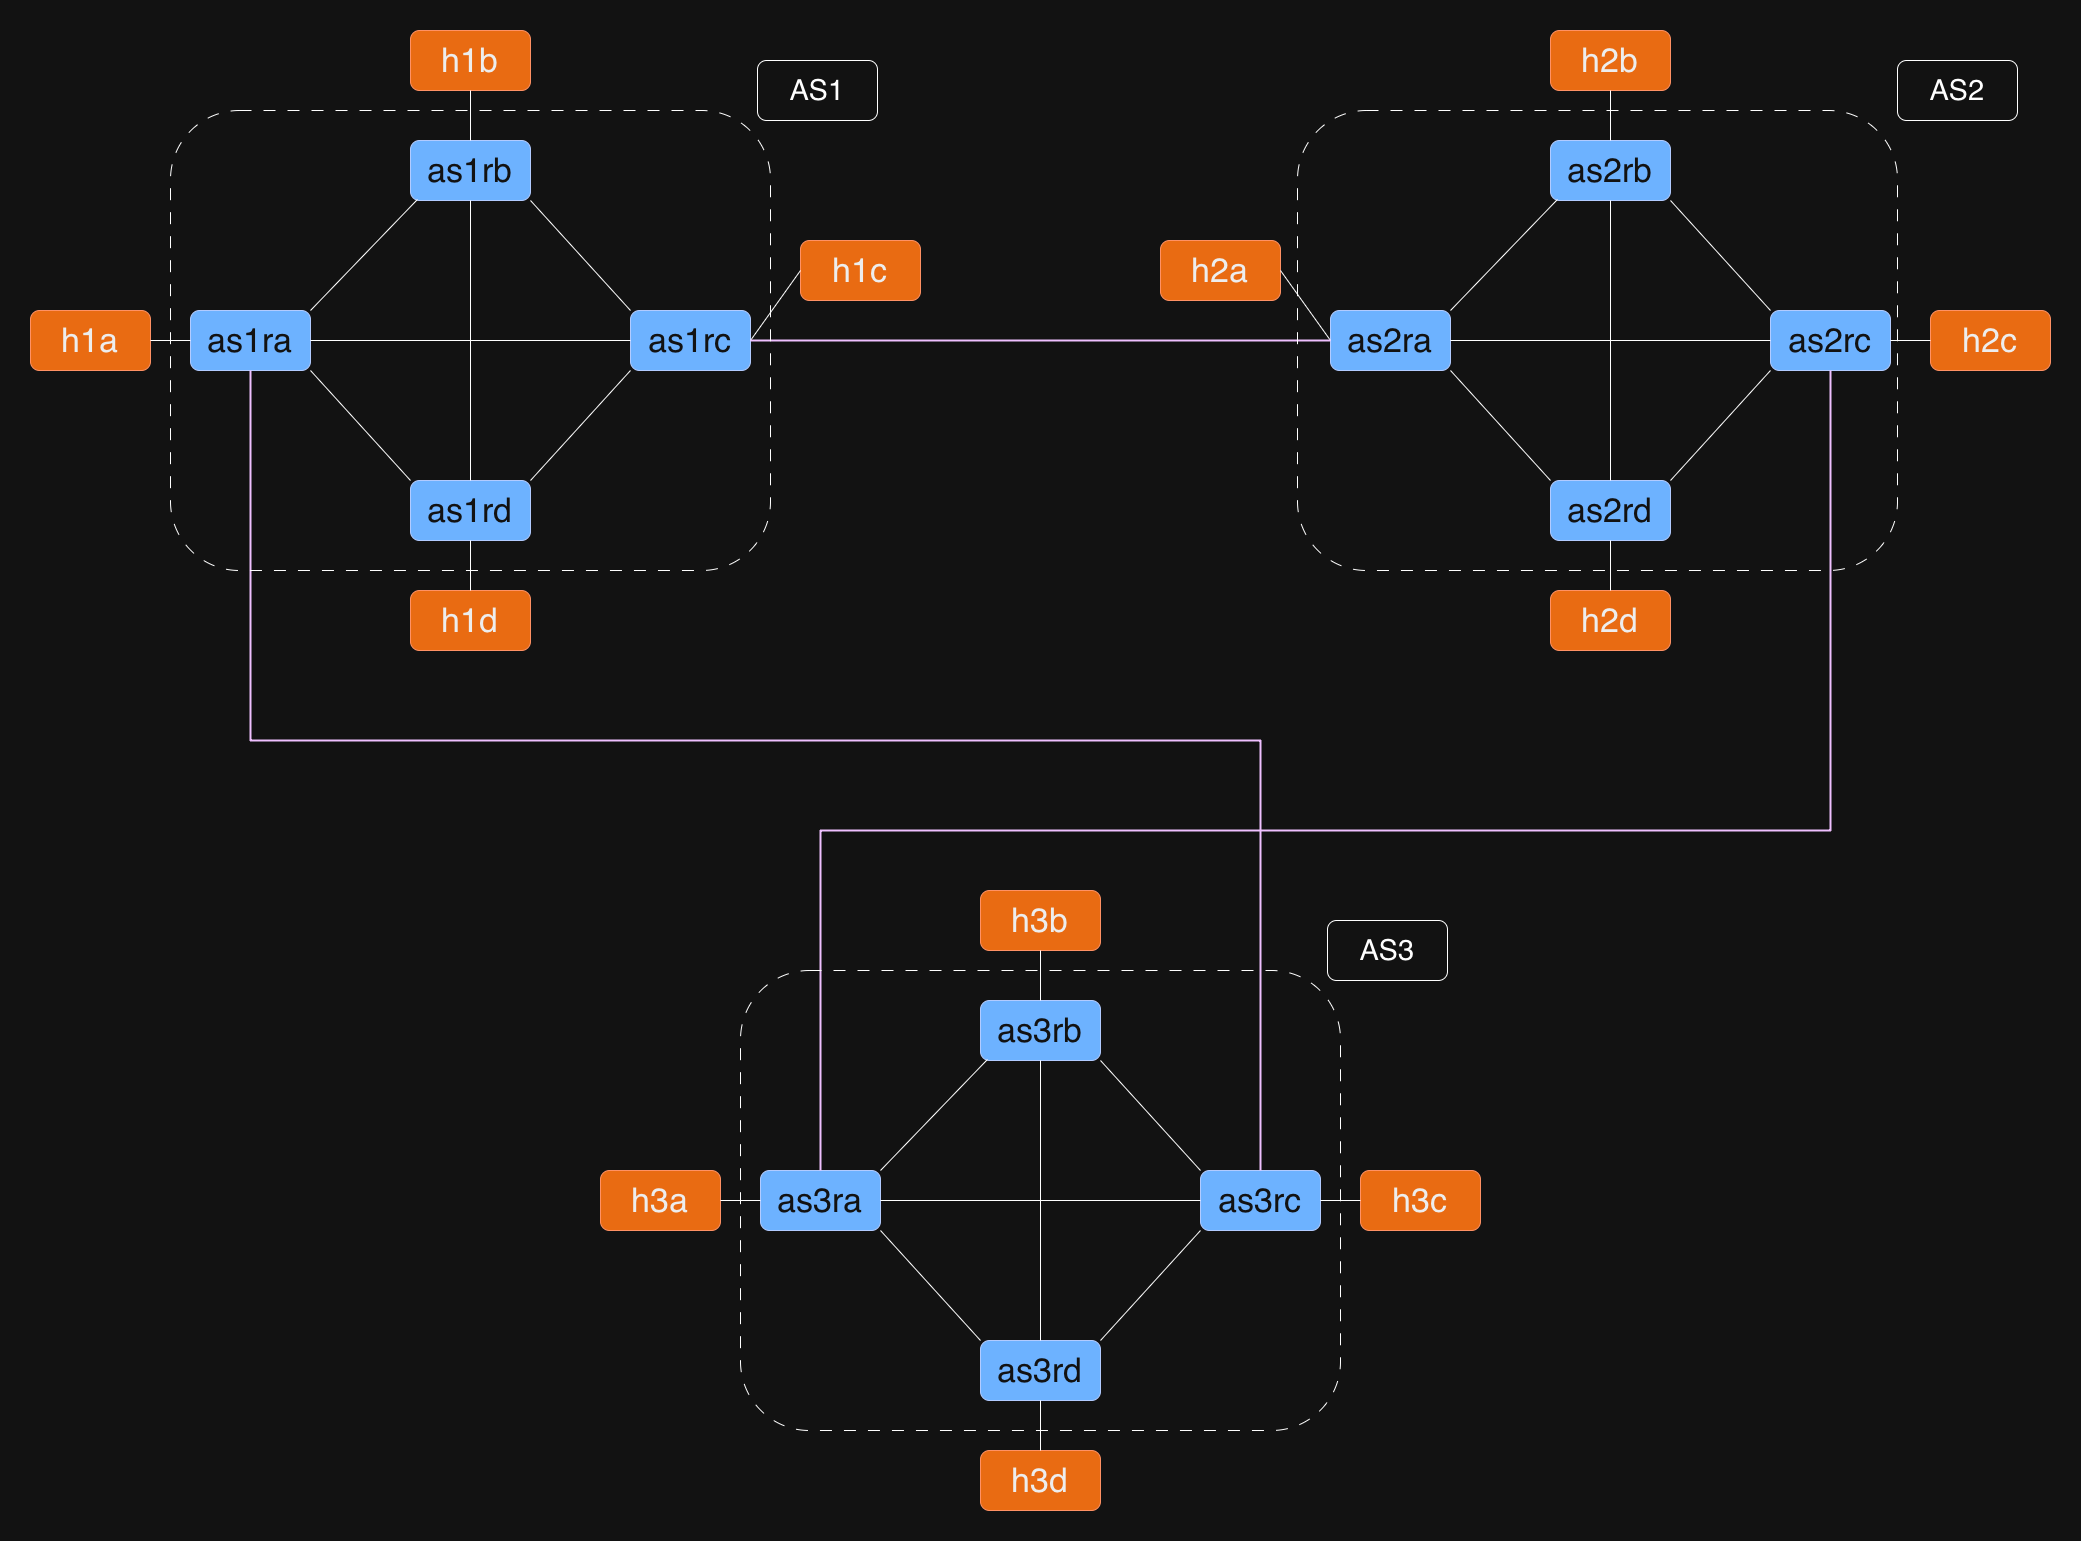
\includegraphics[width=1\textwidth]{traces/L4-3-1.drawio.png}
\end{figure}